\section{実験手法}
%相転移の実験は光学クライオスタット中のヘリウムガス
本章では電流パルスを用いたαスズからβスズへの変換と共存状態生成に関する実験手法について説明する。

\subsection{電流パルスを用いたα相からβ相への変換}
まずパルス印加の前に抵抗の温度依存性も測定した。抵抗の温度依存性を測定するときの電気回路の模式図を図\ref{fig:schematics_lockin}に示す。ロックインアンプ(Stanford Research SR830)から出力した105Hzの交流電圧は、光学クライオスタット中の試料とロード抵抗の直列接続に印加される。回路に流れる電流は$\rm 150\Omega$のロード抵抗の電圧降下をマルチメータ(Keithley 2001)で読み取り算出した。試料の電圧端子間の電圧効果はトランス増幅器(Stanford Research SR554)で100倍に増幅したあと、ロックインアンプの入力端子に入力した。回路に流す電流値は、25Kの試料にパルス電流を印加したとき温度上昇しなかった値より十分小さくとった。また試料の複素インピーダンスの虚部(位相進み/遅れ)成分は実部の1/100程度以下だったので無視して、実部のみを抵抗とした。
\begin{figure}[!h]
     \begin{center}
   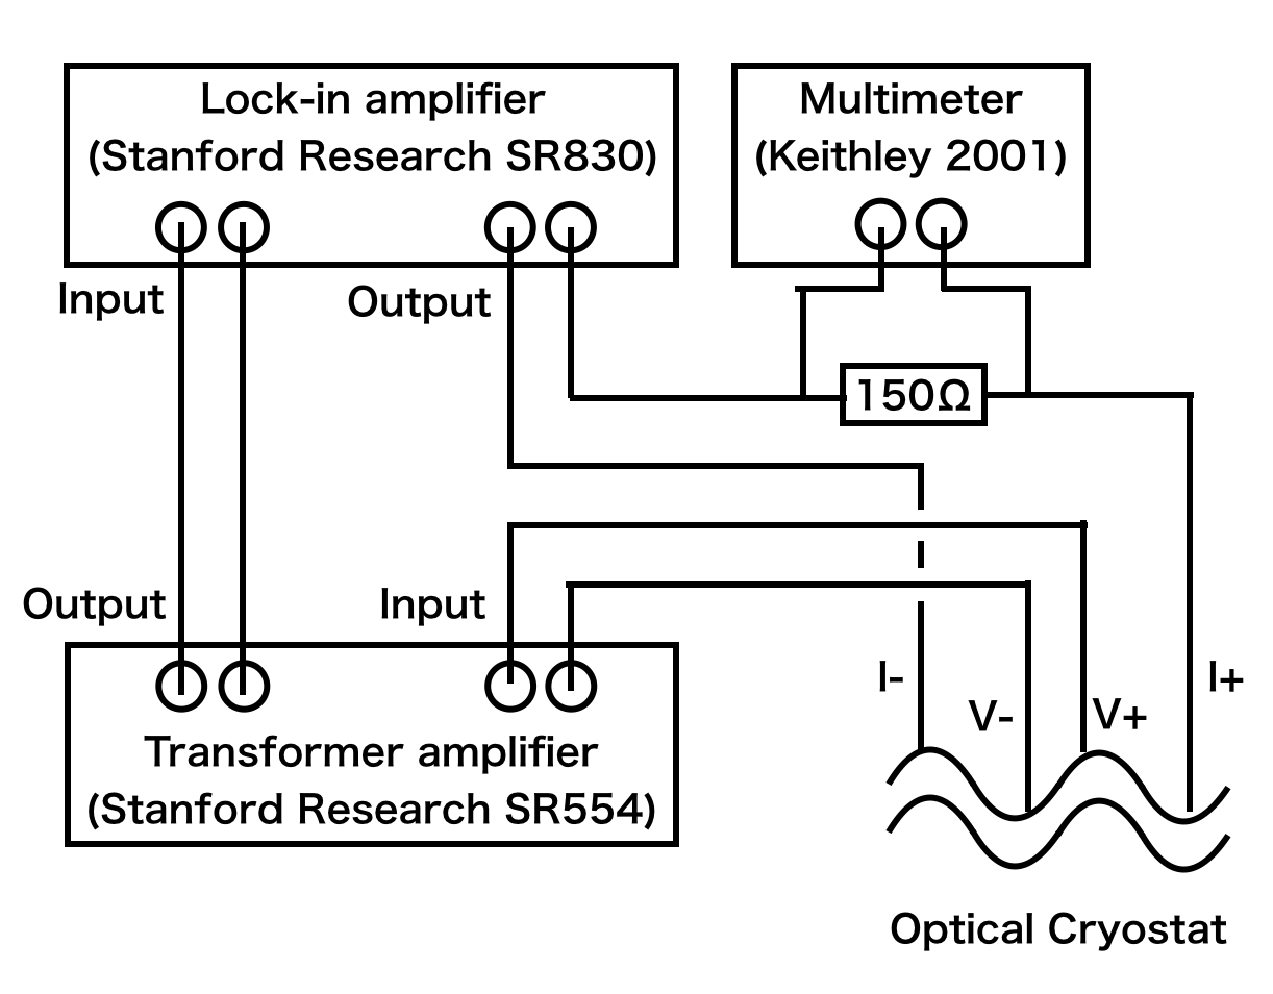
\includegraphics[width=0.5\hsize]{experiment/schematics_lockin.eps}
  \end{center}
  \caption{}
  \label{fig:schematics_lockin}
\end{figure}


抵抗の温度依存性を測定した後αスズからβスズに相転移を起こすことを目的として、25Kに保った試料に孤立した電流パルスを3秒印加してジュール発熱により加熱した。スズ相転移前後で抵抗が大きく異なるため、相転移の確認はパルス印加中の抵抗変化を測定することで行った。その際用いた電気回路の模式図を図\ref{fig:schematics_pulse}に示す。ソースメータ(Keithley 2400)から出力されたパルス電圧は、パワーアンプ(NF Corp. 4502)で100倍に増幅されたあと、光学クライオスタット中の試料とロード抵抗の直列接続に印加される。回路に流れる電流の時間変化は、$\rm 5.4\Omega$のロード抵抗の電圧降下をデータロガー(MC DT8824)で読み取り計算した(Ch2)。また試料の電圧降下もデータロガー(MC DT8824)で読み取り計算した(Ch1)
\begin{figure}[!h]
    \begin{center}
   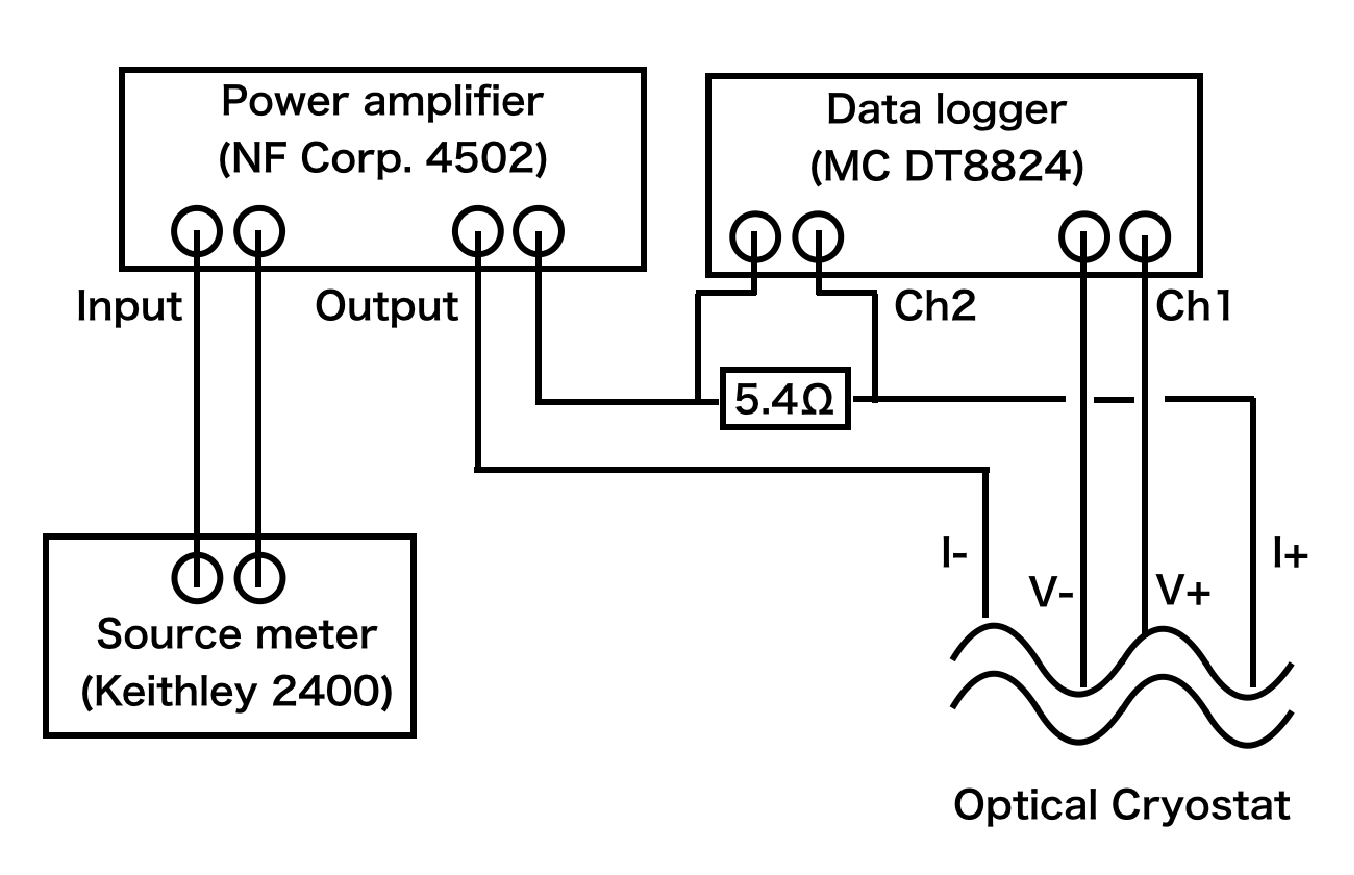
\includegraphics[width=0.5\hsize]{experiment/schematics_pulse.eps}
  \end{center}
  \caption{}
  \label{fig:schematics_pulse}
  \end{figure}
  
効果的に試料を加熱するために筆者は図\ref{fig:schematics_sample}のような端子の接続法を用いた。付録\ref{sec:4terminal}に述べるように、カーボンペーストは発熱に十分に高い抵抗が実現できる一方で機械的な強度が低く、銀ペーストは強度が高い一方で抵抗が小さい。これらを効果的に組み合わせることで、筆者は機械的強度と高抵抗を確保できると筆者は考えた。そこでカーボンペーストで金線をコーティングした後、銀ペーストで覆い試料にしっかりと接続した。この構成では低抵抗率の銀ペーストが挟まっているので試料と金線の間に電流経路が集中せず、比較的一様な発熱が可能となったと考える。また電流端子につなぐ金線は1A程度以下の電流で焼き切れないように直径$\rm 50 \mu m$のものとした。一方、電圧端子をつなぐ線には大電流が流れないため、柔らかく熱伝導の高すぎないものとしたかった。そこで直径$\rm 25 \mu m$の金線とした。
\begin{figure}[!h]
    \begin{center}
   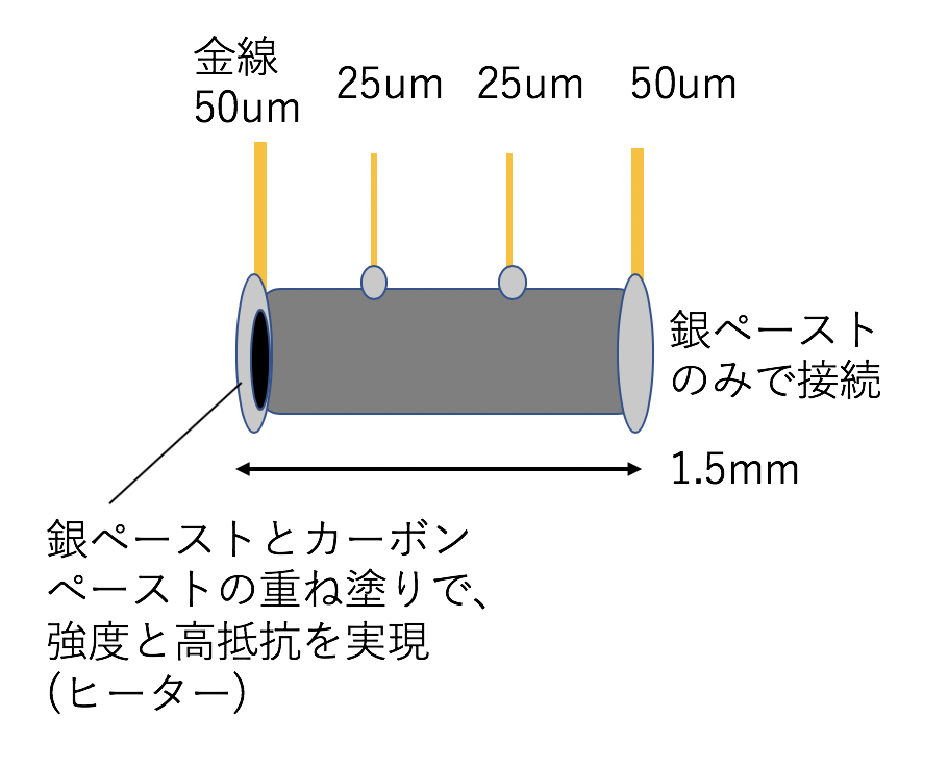
\includegraphics[width=0.4\hsize]{experiment/schematics_sample.eps}
  \end{center}
  \caption{}
  \label{fig:schematics_sample}
\end{figure}

電流パルスを印加した後にふたたび試料抵抗の温度依存性を測定した。パルス印加前と同様に図\ref{fig:schematics_lockin}の電気回路を用いた。

\subsection{電流パルスによるαスズとβスズの共存状態の生成}
次に電流パルスを印加してαスズを部分的にβスズに変換し、αスズとβスズの共存状態を生成することを目指した。序論で述べた通りαスズとβスズはともに温度200K以下と室温で安定である。室温でもパルス印加で相転移が示せれば極めて有用と筆者は考える。さらに低温での実験に比べ冷媒を必要とせず、簡便で実験の自由度も大きい。そこで本実験では室温に保った試料に電流パルスを印加した。

本実験に用いた電気回路は前節のパルス印加実験と同様である。ただし図\ref{fig:schematics_sample2}のように電流端子の片側のみにカーボンペーストを用いた点が異なる。主に片側のみから発熱させることで意図的に試料内の温度勾配を作り出し、部分的な書き込みを制御した。カーボンペーストを用いて接続する方法は前節と同様である(付録\ref{sec:4terminal})。
\begin{figure}[!h]
    \begin{center}
   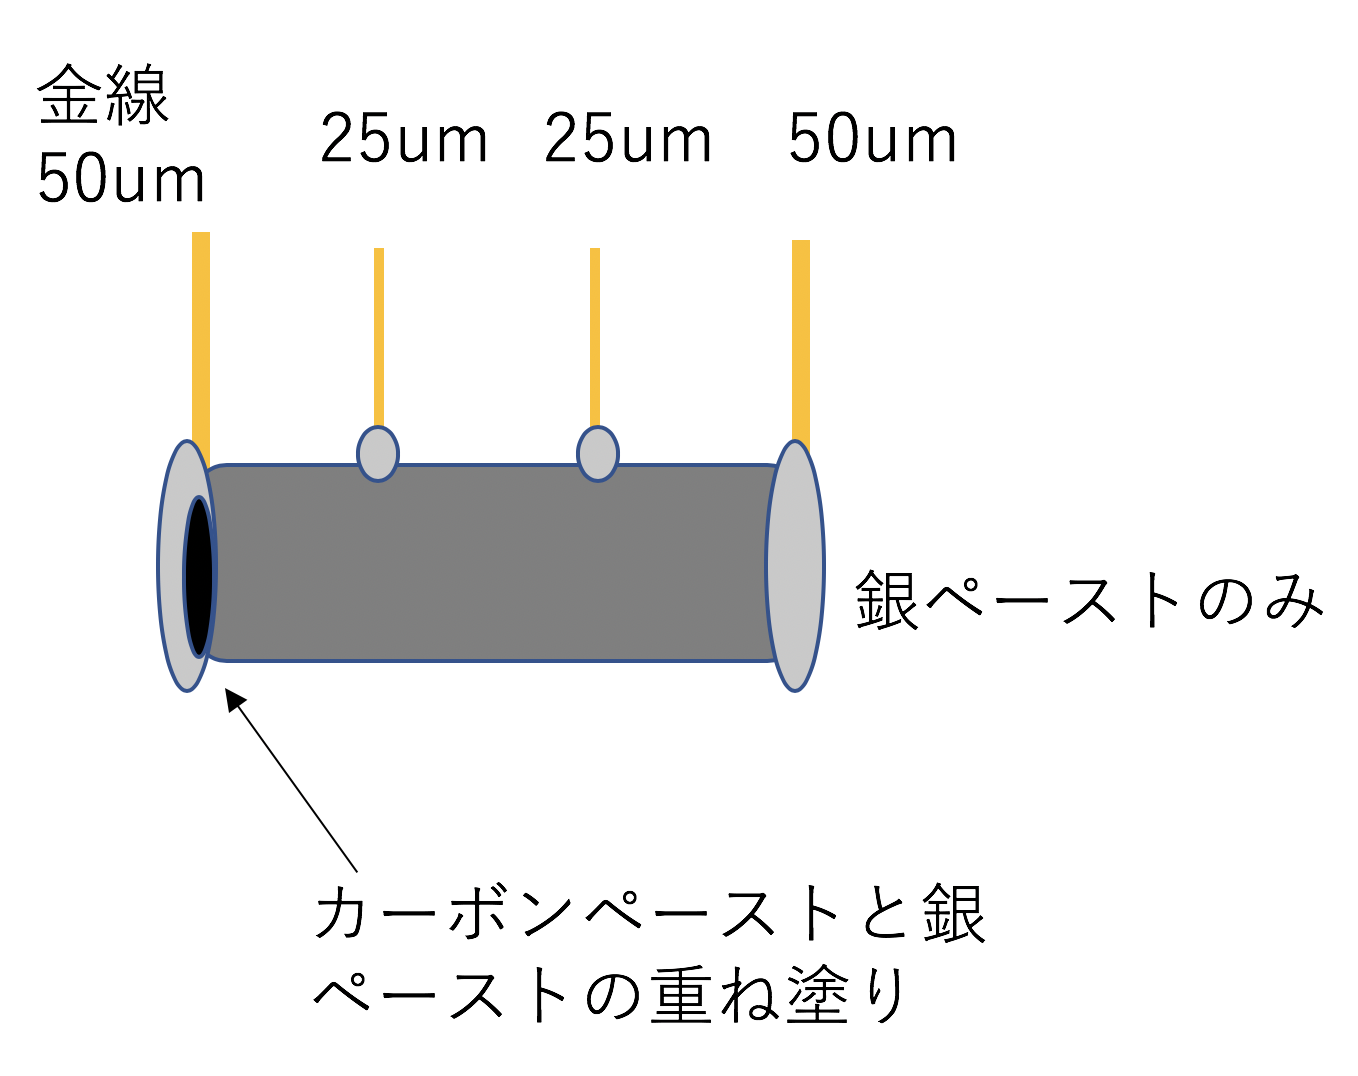
\includegraphics[width=0.4\hsize]{experiment/schematics_sample2.eps}
  \end{center}
  \caption{}
  \label{fig:schematics_sample2}
\end{figure}

また顕微光学系を構成し、パルス印加中の試料を光学的に観察した。図\ref{fig:microscope}に顕微光学系の模式図を示す。光源から照明を入射する際に、顕微光学系の光軸から外した配置とすることで迷光を抑え、コントラストの大きな動画・画像を撮影した。
\begin{figure}[!h]
    \begin{center}
   \includegraphics[width=0.4\hsize]{experiment/microscope.eps}
  \end{center}
  \caption{}
  \label{fig:microscope}
\end{figure}

本実験ではパルス幅1秒、インターバル1秒のパルス列を試料に印加した。

%\subsection{電流パルスを用いたβ相からα相への変換}

\clearpage

%\ref{sec:4terminal}